\section{Data Set}

Briefly describe the data set and cite the main grand challange paper. 

We just need to describe what the data is about. 

\begin{figure}%
	\centering
	\subfloat[point cloud readings simulated for a LiDAR sensor]{{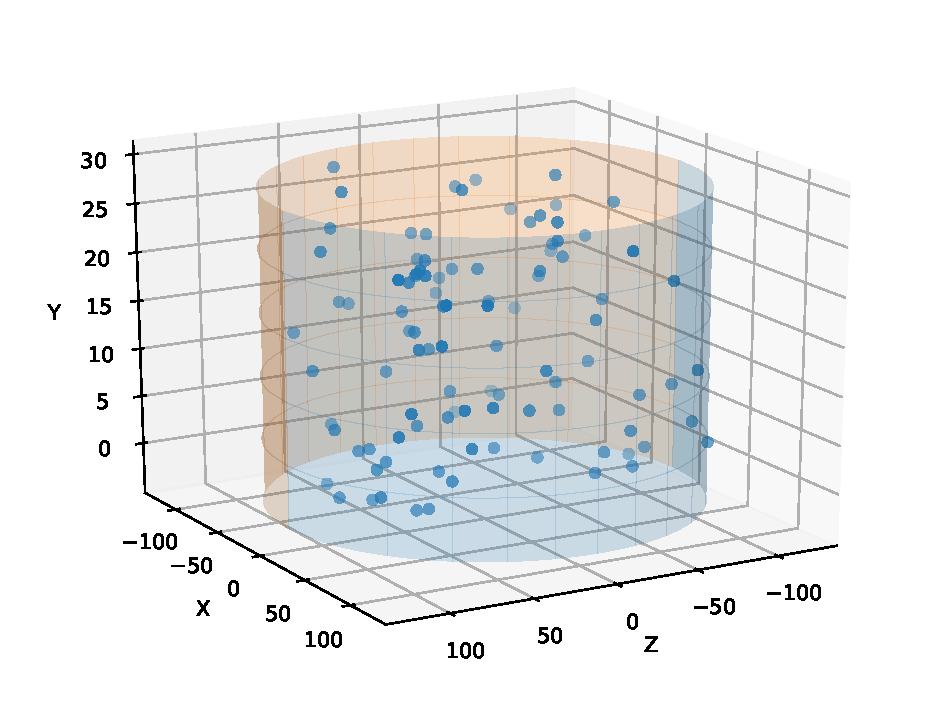
\includegraphics[width=7cm]{images/data_overview.pdf} }}%
	\qquad
	\subfloat[a scene with different numbers of objects]{{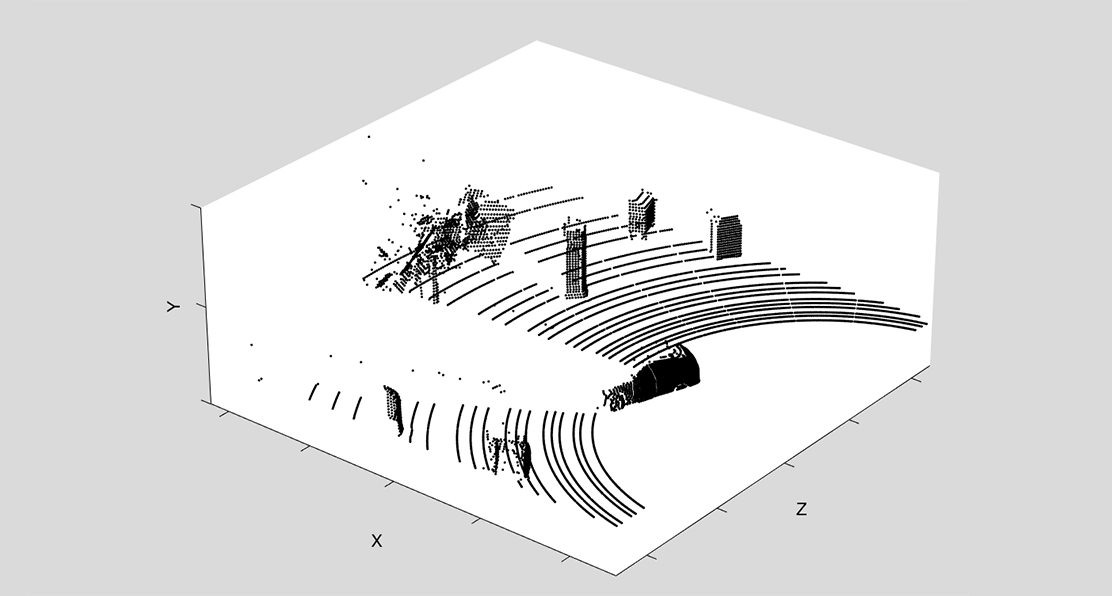
\includegraphics[width=7cm]{images/GC1.png} }}%
	\caption{The data provided consists of point cloud readings simulated for a LiDAR sensor that mounts 64 lasers(a), and Each reading is composed of attributes where X, Y, and Z coordinates are as presented in (b)}%
	\label{fig:data_overview}%
\end{figure}


\cite{DEBSGC2019}



We need to mention other data sets like The KITTI Dataset \cite{Geiger2013IJRR}